\chapter{Diseño}
\label{chap:design}

\section{Diagrama de la arquitectura del sistema}

Como se puede observar en la imagen, la arquitectura del sistema es una arquitectura sencilla. El usuario interacciona únicamente con la interfaz gráfica de la aplicación y la aplicación solicita a la base de datos la información que el usuario requiere. De la misma forma, la base de datos envía la información a la aplicación y la aplicación se la muestra al usuario. El usuario y la base de datos no se relacionan directamente, siempre estará la aplicación como intermediario. 

No es necesaria la existencia de un servidor gracias a la herramienta que se está utilizando como base de datos, Supabase. Esta herramienta da servicio para construir aplicaciones software. 

\begin{figure}[ht]
	\centering
	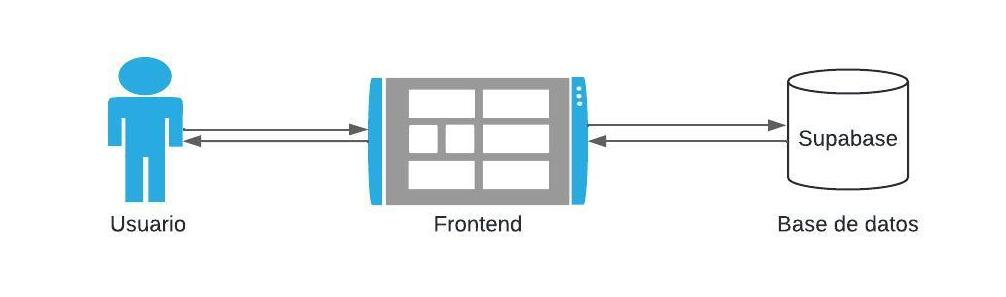
\includegraphics[width=1\textwidth]{imagenes/imagenesDiagramas/DiagramaArquitecturaSistema.jpeg}
	\caption{Diagrama de la arquitectura del sistema.}
	\label{fig:diagArquitectura}
\end{figure}

\newpage

\section{Diseño de la interfaz gráfica}

Debemos buscar la usabilidad y accesibilidad en una aplicación de estas características ya que el usuario final puede no tener grandes destrezas tecnológicas. Por tanto, hay que conseguir un diseño sencillo, fácil de usar e intuitivo. \\

Para ello, habrá que tener en cuenta los siguientes criterios:

\begin{itemize}
	\item \textbf{Botones grandes:} Los botones de la aplicación deben de tener un tamaño adecuado para facilitar la realización de acciones. 
	\item \textbf{Tamaño y contraste del texto:} Nos debemos de asegurar que el tamaño de la letra es lo suficientemente grande y que el contraste con el fondo es significativo para facilitar con ello la lectura. El fondo de la aplicación será blanco para conseguir un buen contraste y evitar las distracciones. 
	\item \textbf{Claridad en la navegación:} Proporcionar una estructura lógica de navegación y unas flechas visibles que permitan cambiar de pantallas de manera intuitiva. 
	\item \textbf{Simplicidad:} El diseño debe ser sencillo. Evitar la sobrecarga de información y priorizar un diseño ordenado. 
	\item \textbf{Feedback:} La aplicación debe proporcionar una respuesta a las acciones del usuario para confirmar que se realizan de manera correcta. 
\end{itemize} 

\newpage

\subsection{Pantalla de inicio de sesión}

En esta sección se muestra el boceto de la interfaz gráfica del inicio de sesión. Se corresponde con el requisito RF1. 

\begin{figure}[ht]
	\centering
	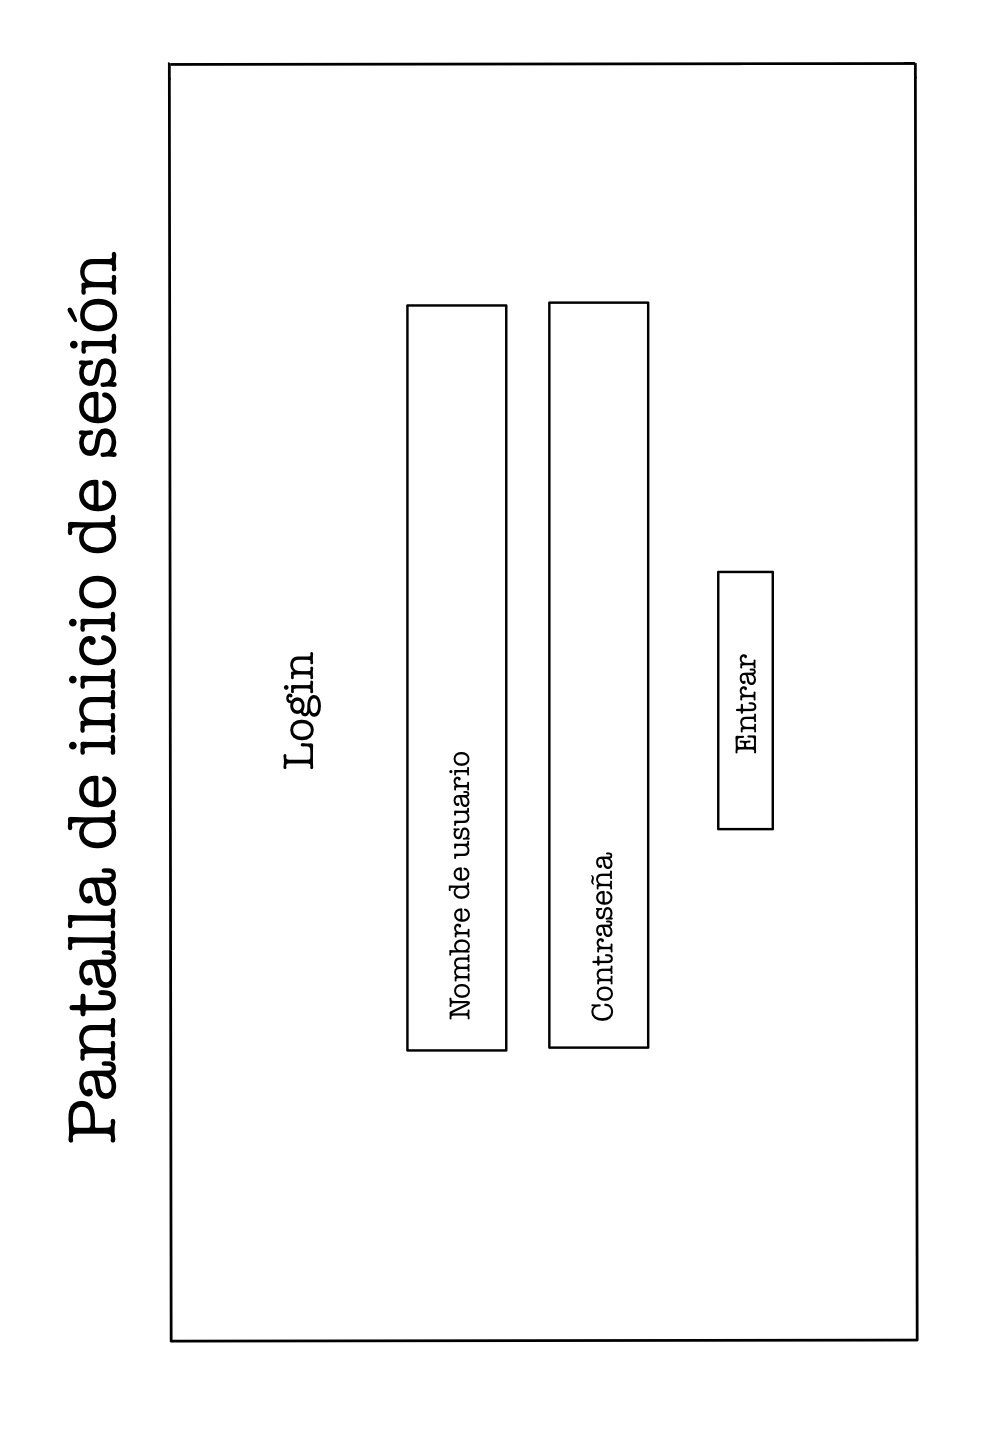
\includegraphics[width=0.7\textwidth, angle=270]{imagenes/inicio_sesion.JPG}
	\caption{Diseño de la pantalla de inicio de sesión.}
	\label{fig:iniciosesion}
\end{figure}

\newpage

\subsection{Pantalla principal}

En esta sección se muestran los bocetos de la interfaz gráfica de la pantalla principal y las pantallas correspondientes con una nueva venta y un nuevo préstamo. Estas tres pantallas representan los requisitos RF19, RF20 y RF28. Por tanto, es la pantalla que muestra la caja diaria y permite registrar una nueva venta o un nuevo préstamo. 

\begin{figure}[ht]
	\centering
	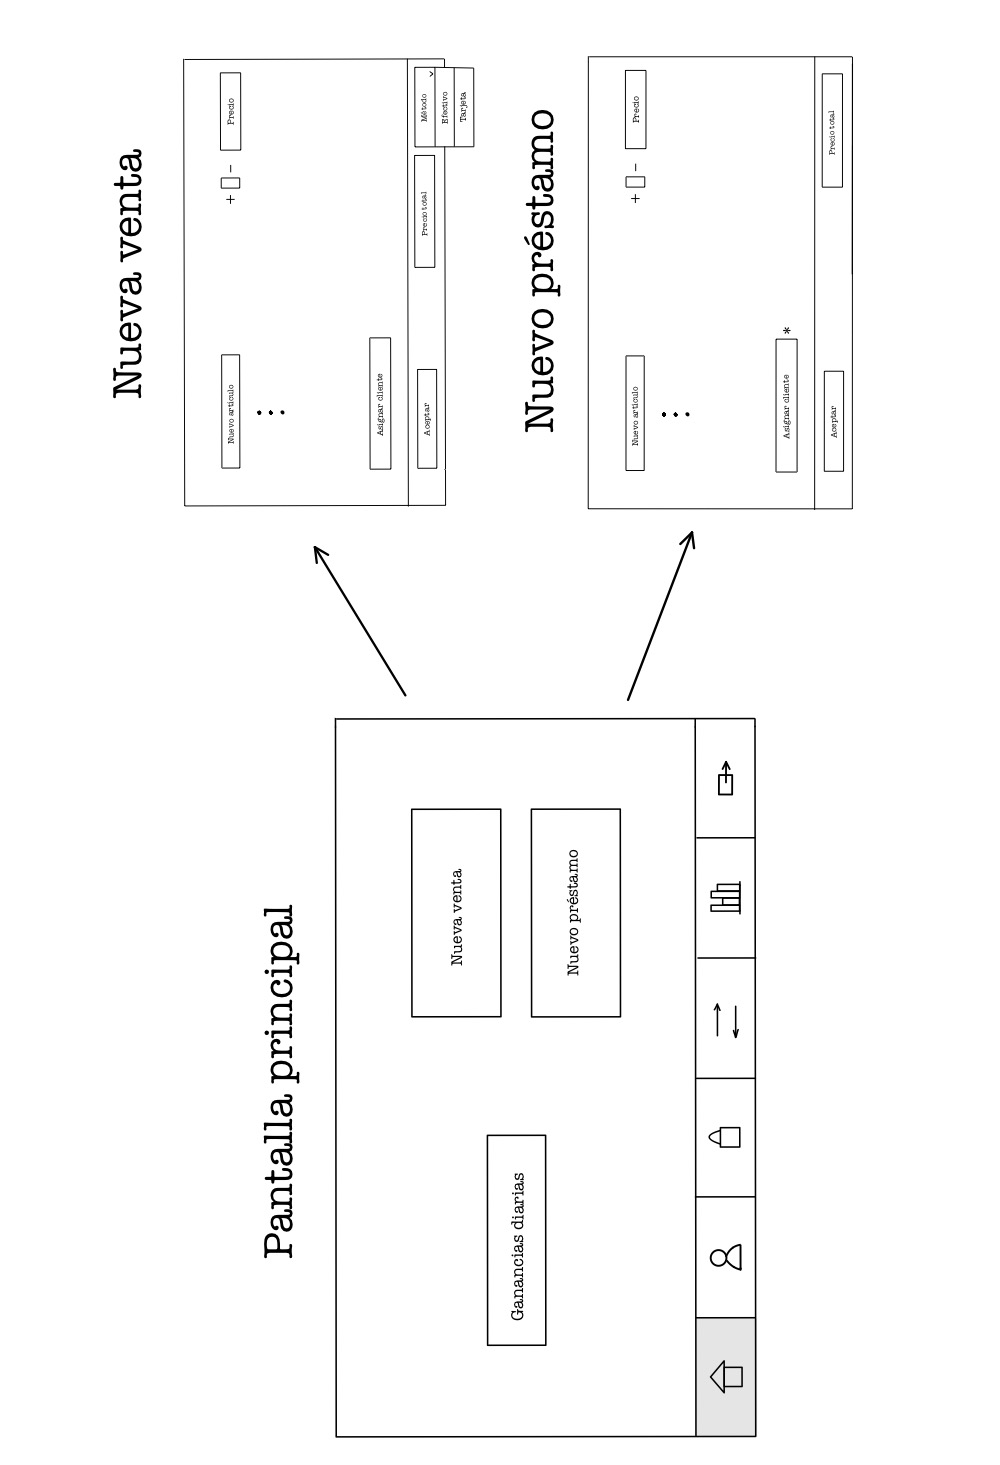
\includegraphics[width=0.8\textwidth, angle=270]{imagenes/pantalla_principal.JPG}
	\caption{Diseño de la pantalla principal.}
	\label{fig:pantallaprincipal}
\end{figure}

\newpage

\subsection{Pantalla de clientes}

En esta sección se muestran los bocetos de la interfaz gráfica de la pantalla clientes. Estas cuatro pantallas representan los requisitos RF12, RF13, RF14, RF15, RF16, RF17 y RF18. En la pantalla clientes podemos ver la lista de clientes existentes, buscar clientes por nombre y filtrar aquellos clientes que tengan préstamos. Si pulsamos encima del nombre del cliente, visualizaremos todos los datos relacionados con este. Además, podemos editar, eliminar y añadir un nuevo cliente. 


\begin{figure}[ht]
	\centering
	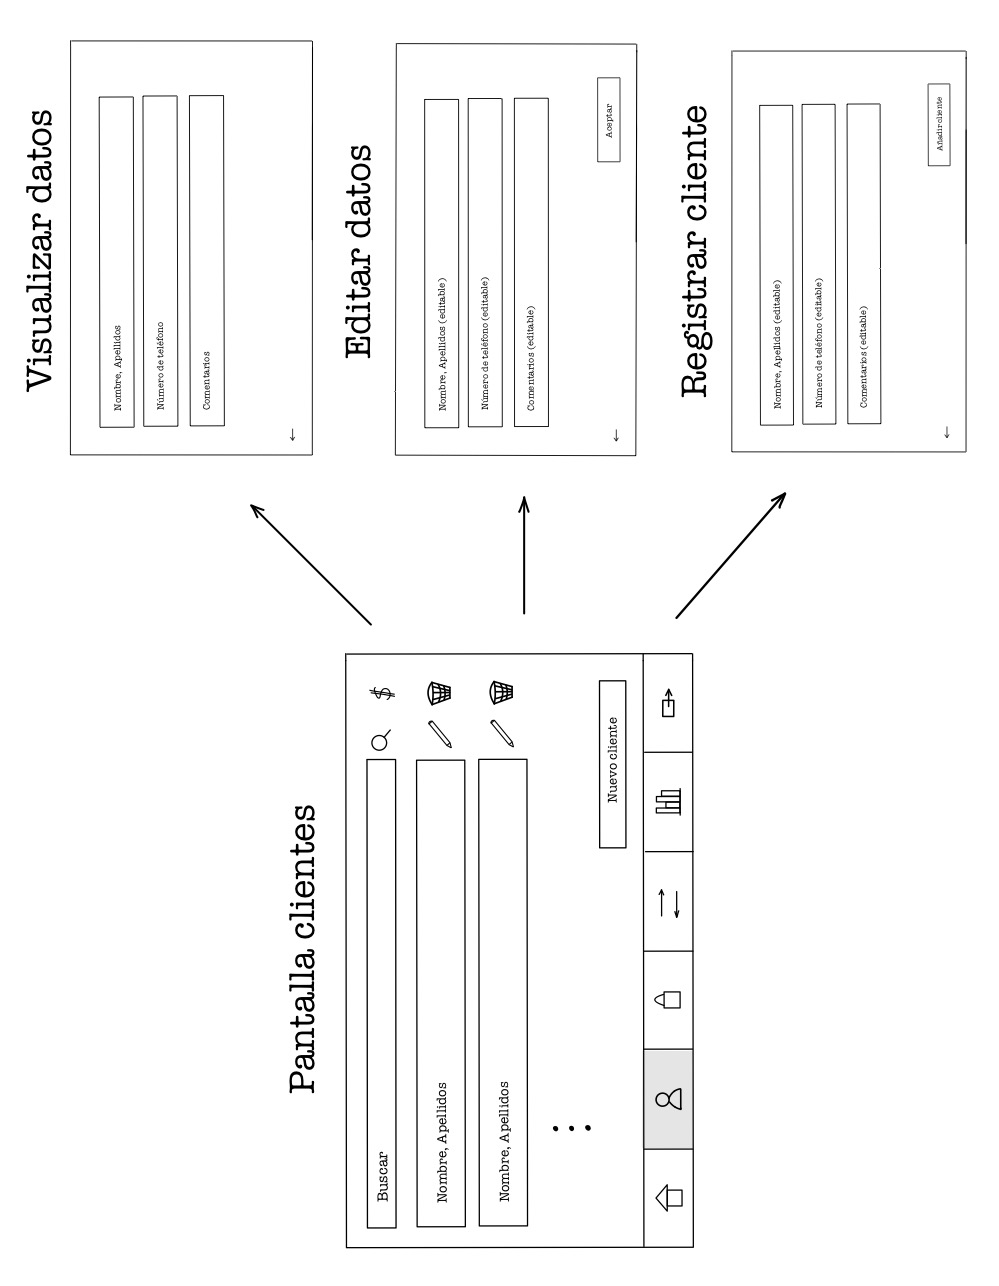
\includegraphics[width=0.8\textwidth, angle=270]{imagenes/pantalla_clientes.JPG}
	\caption{Diseño de la pantalla clientes.}
	\label{fig:pantallaclientes}
\end{figure}

\newpage

\subsection{Pantalla de artículos}

En esta sección se muestran los bocetos de la interfaz gráfica de la pantalla artículos. Estas cinco pantallas representan los requisitos RF3, RF4, RF5, RF6, RF7, RF8, RF9, RF10 y RF11. En la pantalla artículos podemos ver la lista de artículos existentes, buscar los artículos por nombre y filtrarlos por categoría. Si pulsamos encima del nombre del artículo, visualizaremos todos los datos relacionados con este. Además, podemos editar, eliminar y añadir un nuevo artículo. Por último, tenemos la lista de renovación de stock donde se introducirán todos los artículos que deba comprar el comerciante. 


\begin{figure}[ht]
	\centering
	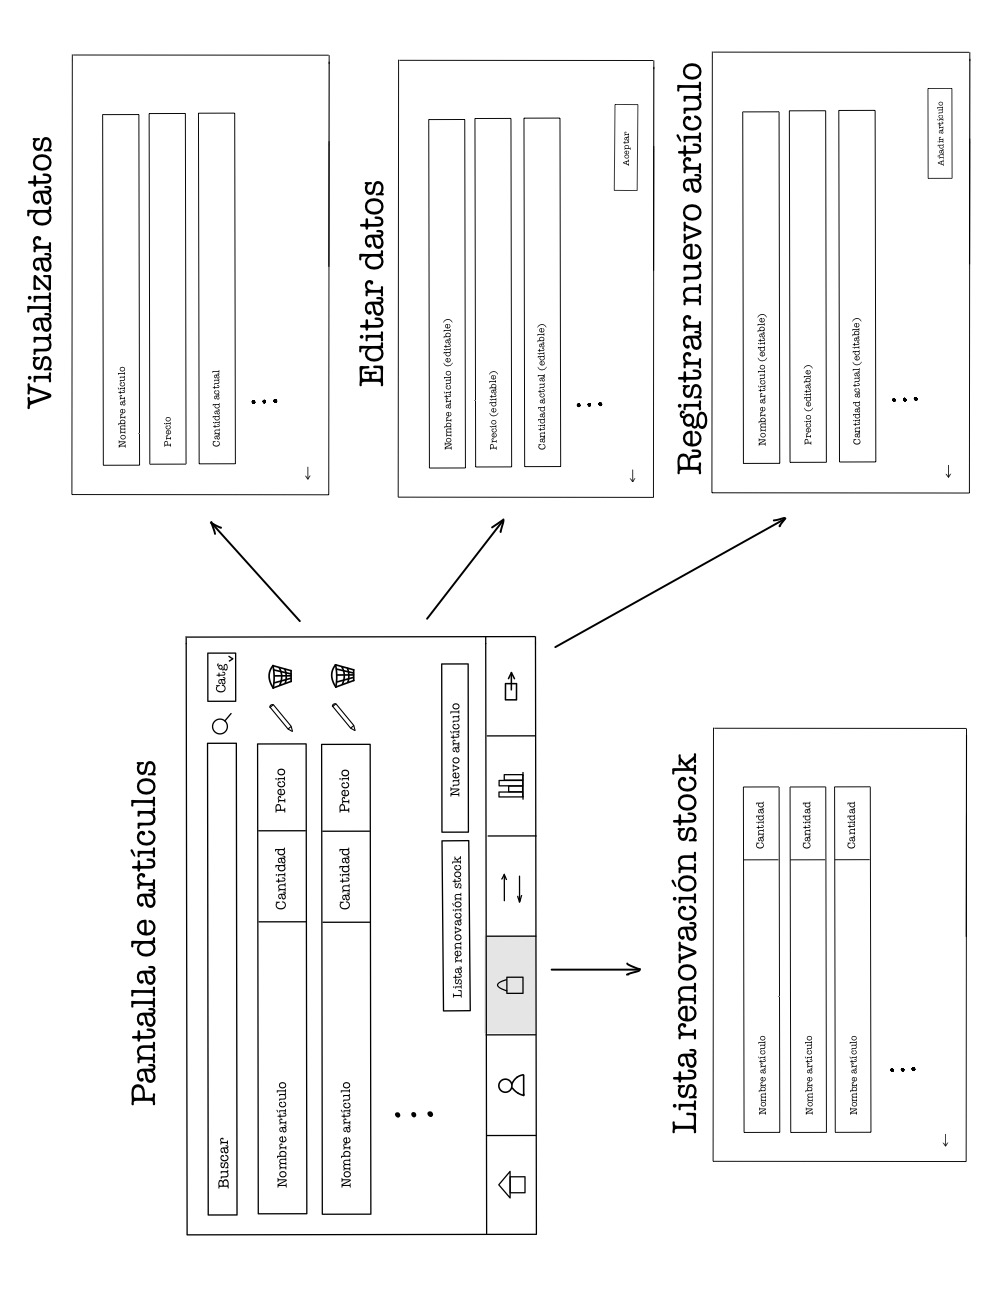
\includegraphics[width=0.8\textwidth, angle=270]{imagenes/pantalla_articulos.JPG}
	\caption{Diseño de la pantalla artículos.}
	\label{fig:pantallaarticulos}
\end{figure}

\newpage


\subsection{Pantalla de movimientos}

En esta sección se muestran los bocetos de la interfaz gráfica de la pantalla movimientos. Estas cuatro pantallas representan los requisitos RF21, RF22, RF23, RF24, RF25, RF26 y RF27. En la pantalla movimientos podemos ver la lista de movimientos existentes, buscar los movimientos por fecha o cliente asignado y filtrarlos por tipo de movimiento (venta, préstamo o devolución). Si pulsamos encima del movimiento, visualizaremos todos los datos relacionados con este. Si el movimiento es de tipo "préstamo", además de visualizarlo podremos convertirlo en venta seleccionando aquellos artículos que el cliente desea comprar. Únicamente se podrán devolver las ventas, ya que son los movimientos que generan una subida económica en la caja diaria. Las devoluciones generan una bajada correspondiente con la cantidad devuelta. Si se devuelve un préstamo sin comprar nada, se elimina el movimiento. Podemos eliminar cualquier movimiento, sea del tipo que sea. 


\begin{figure}[ht]
	\centering
	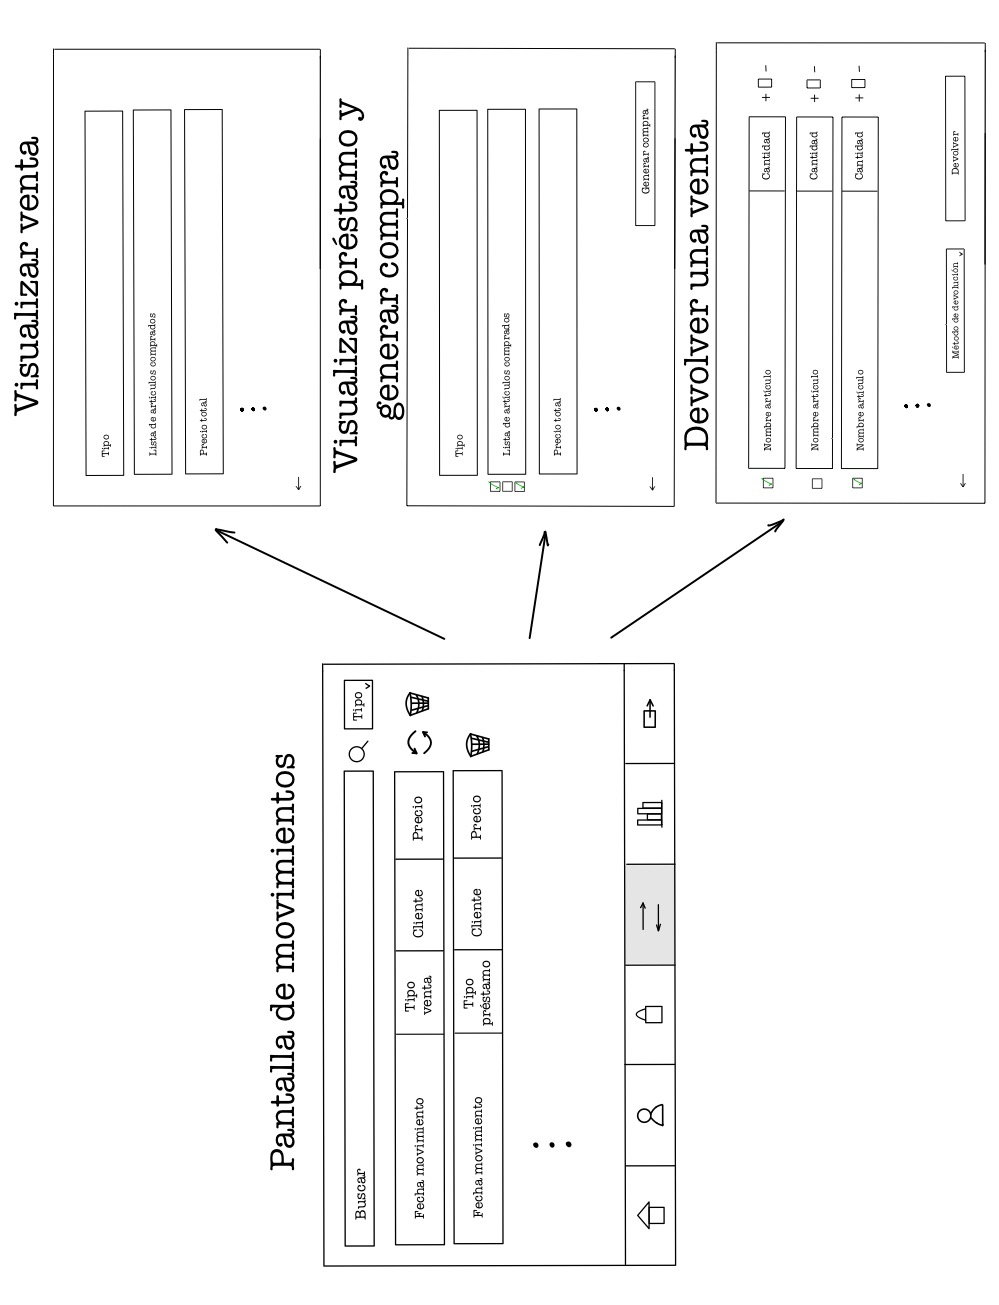
\includegraphics[width=0.8\textwidth, angle=270]{imagenes/pantalla_movimientos.JPG}
	\caption{Diseño de la pantalla movimientos.}
	\label{fig:pantallamovimientos}
\end{figure}

\newpage

\subsection{Pantalla de gráficos y cierre de sesión}

En esta sección se muestra el boceto de la interfaz gráfica de la pantalla gráficos. Esta pantalla representa el requisito RF29. Aquí podemos observar el progreso económico del negocio en forma de gráfica. Podremos verlo de forma mensual o anual. 

Para finalizar, el cierre de sesión podrá hacerse desde cualquier lugar simplemente pulsando en su botón. Esto corresponde con el requisito RF2. 


\begin{figure}[ht]
	\centering
	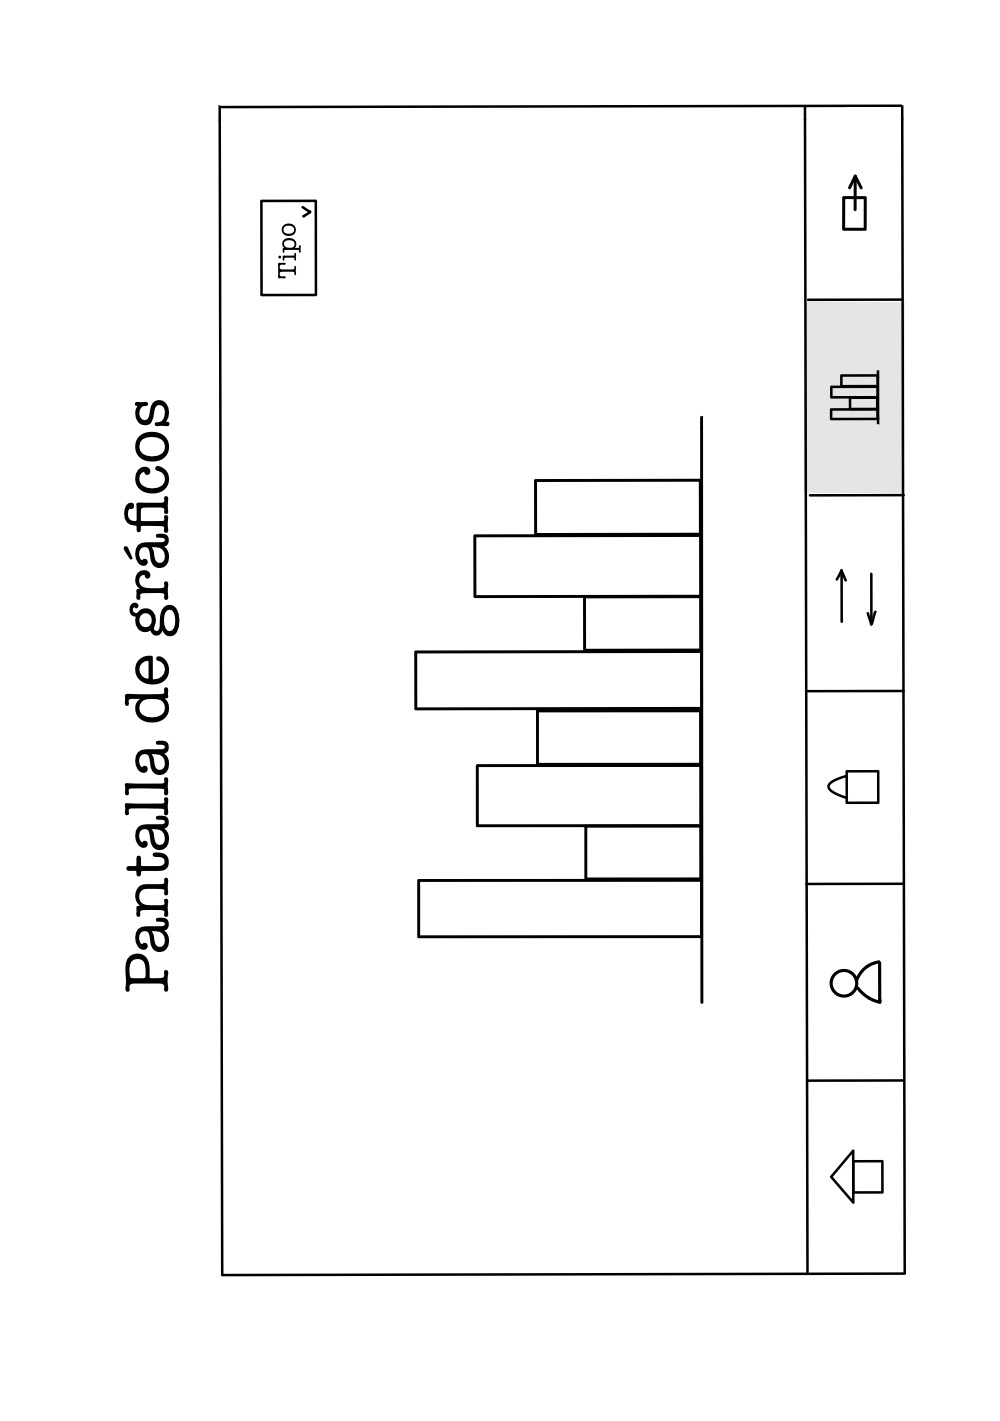
\includegraphics[width=0.8\textwidth, angle=270]{imagenes/pantalla_graficos.JPG}
	\caption{Diseño de la pantalla gráficos.}
	\label{fig:pantallagraficos}
\end{figure}